\documentclass{article}

% content/resources/templates/preamble.tex
\usepackage[margin=0.6in]{geometry}
\author{Milav Dabgar}
\usepackage{amsmath,amssymb,amsthm}
\usepackage{booktabs}
\usepackage{multirow}
\usepackage{xcolor}
\usepackage{tcolorbox}
\tcbuselibrary{breakable,skins}
\usepackage[colorlinks=true,linkcolor=blue]{hyperref}
\usepackage{titlesec}
\usepackage{enumitem}
\usepackage{tikz}
\usepackage{pgfplots}
\usepackage{circuitikz}
\usepackage[version=4]{mhchem}
\usepackage{longtable}
\usepackage{array}
\usepackage{float}
\usepackage{caption}
\usepackage{listings}

\lstset{
  basicstyle=\small\ttfamily,
  breaklines=true,
  breakatwhitespace=false,
  postbreak=\mbox{\textcolor{red}{$\hookrightarrow$}\space},
  float=false,
  numbers=left,
  numberstyle=\tiny\color{gray},
  numbersep=10pt,
  xleftmargin=2em,
  keywordstyle=\color{blue},
  commentstyle=\color{green!60!black},
  stringstyle=\color{purple},
  backgroundcolor=\color{gray!5},
  showstringspaces=false,
  tabsize=2,
  captionpos=b,
  keepspaces=true,
  columns=flexible
}

\pgfplotsset{compat=1.18}
\usetikzlibrary{shapes,arrows,positioning,calc,patterns,decorations.pathmorphing,decorations.markings,arrows.meta}

% Color scheme
\definecolor{headcolor}{RGB}{0,102,204}
\definecolor{keycolor}{RGB}{220,20,60}
\definecolor{solutioncolor}{RGB}{34,139,34}
\definecolor{mnemoniccolor}{RGB}{148,0,211}
\definecolor{codecolor}{RGB}{0,0,100}

% Spacing
\setlength{\parskip}{3pt}
\setlist[itemize]{nosep}
\setlist[enumerate]{nosep}

% Title formatting
\titleformat{\section}{\Large\bfseries\color{headcolor}}{\thesection}{1em}{}
\titleformat{\subsection}{\large\bfseries\color{headcolor}}{\thesubsection}{1em}{}

% Pandoc tightlist compatibility
\providecommand{\tightlist}{%
  \setlength{\itemsep}{0pt}\setlength{\parskip}{0pt}}

% Pandoc longtable compatibility
\newcounter{none}
\def\thenone{}


% content/resources/templates/english-boxes.tex

% Custom environments
\newtcolorbox{solutionbox}{
 breakable,
 enhanced,
 colback=solutioncolor!5!white,
 colframe=solutioncolor!75!black,
 fonttitle=\bfseries,
 title=Solution
}

\newtcolorbox{solutionboxnobreak}{
 colback=solutioncolor!5!white,
 colframe=solutioncolor!75!black,
 fonttitle=\bfseries,
 title=Solution
}

\newtcolorbox{keyformula}{
 breakable,
 enhanced,
 colback=keycolor!5!white,
 colframe=keycolor!75!black,
 fonttitle=\bfseries,
 title=Key Formula
}

\newtcolorbox{mnemonicboxenv}{
 breakable,
 enhanced,
 colback=mnemoniccolor!5!white,
 colframe=mnemoniccolor!75!black,
 fonttitle=\bfseries,
 title=Mnemonic
}

\newcommand{\mnemonicbox}[1]{%
  \begin{mnemonicboxenv}
    #1
  \end{mnemonicboxenv}
}


% Custom commands for GTU solutions
% This file defines semantic commands for consistent formatting

% Question command with automatic formatting
\newcommand{\question}[2]{%
  \section*{Question #1}%
  \textbf{#2}%
}

% OR question variant
\newcommand{\questionor}[2]{%
  \section*{Question #1 OR}%
  \textbf{#2}%
}

% Proper table environment with caption
\newenvironment{answertable}[1]{%
  \begin{table}[htbp]
  \centering
  \caption{#1}
}{%
  \end{table}
}

% Proper figure environment for diagrams
\newenvironment{answerdiagram}[1]{%
  \begin{figure}[htbp]
  \centering
  \caption{#1}
}{%
  \end{figure}
}

% Semantic markup for key terms
\newcommand{\keyword}[1]{\textbf{#1}}
\newcommand{\code}[1]{\texttt{#1}}
\newcommand{\classname}[1]{\texttt{#1}}
\newcommand{\methodname}[1]{\texttt{#1}}

% Proper quotation marks
\newcommand{\mnemonic}[1]{``#1''}


\title{Microprocessor \& Microcontroller Systems (1333202) - Winter 2024 Solution}
\date{December 05, 2024}

\begin{document}
\maketitle

\questionmarks{1(a)}{3}{List the features of 8051 Microcontroller.}

\begin{solutionbox}
The 8051 microcontroller has several important features:

\begin{center}
\captionof{table}{Features of 8051}
\begin{tabulary}{\linewidth}{|L|L|}
\hline
\textbf{Feature} & \textbf{Description} \\ \hline
\textbf{CPU} & 8-bit CPU optimized for control applications \\ \hline
\textbf{Memory} & 4KB internal ROM, 128 bytes internal RAM \\ \hline
\textbf{I/O Ports} & 4 bidirectional 8-bit I/O ports (P0-P3) \\ \hline
\textbf{Timers} & Two 16-bit timer/counters (Timer 0 \& Timer 1) \\ \hline
\textbf{Interrupts} & 5 interrupt sources with 2 priority levels \\ \hline
\textbf{Serial Port} & Full duplex UART for serial communication \\ \hline
\end{tabulary}
\end{center}
\end{solutionbox}

\begin{mnemonicbox}
\mnemonic{CPU Memory Input-Output Timers Interrupts Serial (C-MIT-IS)}
\end{mnemonicbox}

\questionmarks{1(b)}{4}{Define: Opcode, Operand, Instruction cycle, Machine cycle}

\begin{solutionbox}
\begin{center}
\captionof{table}{Definitions}
\begin{tabulary}{\linewidth}{|L|L|}
\hline
\textbf{Term} & \textbf{Definition} \\ \hline
\textbf{Opcode} & Operation code that specifies the operation to be performed \\ \hline
\textbf{Operand} & Data or address on which the operation is performed \\ \hline
\textbf{Instruction Cycle} & Complete process of fetching, decoding and executing an instruction \\ \hline
\textbf{Machine Cycle} & Time required to access memory or I/O device \\ \hline
\end{tabulary}
\end{center}

\begin{center}
\begin{tikzpicture}[node distance=2cm, auto]
    \node [gtu state] (fetch) {Fetch};
    \node [gtu state, right=of fetch] (decode) {Decode};
    \node [gtu state, right=of decode] (execute) {Execute};
    
    \draw [gtu arrow] (fetch) -- (decode);
    \draw [gtu arrow] (decode) -- (execute);
    \draw [gtu arrow] (execute) to[bend left=45] (fetch);
\end{tikzpicture}
\captionof{figure}{Instruction Cycle}
\end{center}
\end{solutionbox}

\begin{mnemonicbox}
\mnemonic{Opcode Operand Instruction-cycle Data-cycle (OOID)}
\end{mnemonicbox}

\questionmarks{1(c)}{7}{Compare Von Neumann and Harvard Architecture.}

\begin{solutionbox}
\begin{center}
\captionof{table}{Von Neumann vs Harvard}
\begin{tabulary}{\linewidth}{|L|L|L|}
\hline
\textbf{Parameter} & \textbf{Von Neumann} & \textbf{Harvard} \\ \hline
\textbf{Memory Structure} & Single memory for program and data & Separate memory for program and data \\ \hline
\textbf{Bus System} & Single bus system & Separate bus for program and data \\ \hline
\textbf{Speed} & Slower due to bus conflicts & Faster simultaneous access \\ \hline
\textbf{Cost} & Lower cost & Higher cost \\ \hline
\textbf{Complexity} & Simple design & Complex design \\ \hline
\textbf{Examples} & 8085, x86 processors & 8051, DSP processors \\ \hline
\end{tabulary}
\end{center}

\begin{center}
\begin{tikzpicture}[node distance=1.5cm]
    % Von Neumann
    \node [gtu block, minimum width=2.5cm] (cpu1) {CPU};
    \node [gtu block, minimum width=2.5cm, below=1.5cm of cpu1] (mem1) {Memory\\(Program + Data)};
    \draw [gtu arrow, <->] (cpu1) -- node[right, font=\small] {Single Bus} (mem1);
    \node [above=0.2cm of cpu1, font=\bfseries] {Von Neumann};

    % Harvard
    \node [gtu block, minimum width=2.5cm, right=4cm of cpu1] (cpu2) {CPU};
    \node [gtu block, below right=1.5cm of cpu2] (dmem) {Data\\Memory};
    \node [gtu block, below left=1.5cm of cpu2] (pmem) {Program\\Memory};
    \draw [gtu arrow, <->] (cpu2) -- node[right, font=\small, pos=0.5] {Data Bus} (dmem);
    \draw [gtu arrow, <->] (cpu2) -- node[left, font=\small, pos=0.5] {Program Bus} (pmem);
    \node [above=0.2cm of cpu2, font=\bfseries] {Harvard};
\end{tikzpicture}
\captionof{figure}{Architecture Comparison}
\end{center}
\end{solutionbox}

\begin{mnemonicbox}
\mnemonic{Von-Single-Bus-Simple-Cheap vs Harvard-Separate-Dual-Fast-Complex (VSBSC vs HSDFC)}
\end{mnemonicbox}

\questionmarks{1(c) OR}{7}{Compare RISC and CISC.}

\begin{solutionbox}
\begin{center}
\captionof{table}{RISC vs CISC}
\begin{tabulary}{\linewidth}{|L|L|L|}
\hline
\textbf{Parameter} & \textbf{RISC} & \textbf{CISC} \\ \hline
\textbf{Instruction Set} & Reduced, simple instructions & Complex instruction set \\ \hline
\textbf{Instruction Size} & Fixed size instructions & Variable size instructions \\ \hline
\textbf{Execution Time} & Single clock cycle per instruction & Multiple clock cycles \\ \hline
\textbf{Memory Access} & Load/Store architecture & Memory-to-memory operations \\ \hline
\textbf{Compiler} & Complex compiler required & Simple compiler \\ \hline
\textbf{Examples} & ARM, MIPS & 8085, x86 \\ \hline
\end{tabulary}
\end{center}

\begin{center}
\begin{tikzpicture}[node distance=1.5cm]
    % RISC Flow
    \node [gtu block] (risc_inst) {Simple\\Instructions};
    \node [gtu block, below=0.8cm of risc_inst] (risc_exec) {Fast\\Execution};
    \node [gtu block, below=0.8cm of risc_exec] (risc_comp) {Complex\\Compiler};
    \draw [gtu arrow] (risc_inst) -- (risc_exec);
    \draw [gtu arrow] (risc_exec) -- (risc_comp);
    \node [above=0.2cm of risc_inst, font=\bfseries] {RISC};

    % CISC Flow
    \node [gtu block, right=4cm of risc_inst] (cisc_inst) {Complex\\Instructions};
    \node [gtu block, below=0.8cm of cisc_inst] (cisc_exec) {Slow\\Execution};
    \node [gtu block, below=0.8cm of cisc_exec] (cisc_comp) {Simple\\Compiler};
    \draw [gtu arrow] (cisc_inst) -- (cisc_exec);
    \draw [gtu arrow] (cisc_exec) -- (cisc_comp);
    \node [above=0.2cm of cisc_inst, font=\bfseries] {CISC};
\end{tikzpicture}
\captionof{figure}{RISC vs CISC Concepts}
\end{center}
\end{solutionbox}

\begin{mnemonicbox}
\mnemonic{Simple-Fast-Complex vs Complex-Slow-Simple (RISC-SFS vs CISC-CSS)}
\end{mnemonicbox}

\questionmarks{2(a)}{3}{List the 16-bit Registers available in 8085 and Explain its Function.}

\begin{solutionbox}
\begin{center}
\captionof{table}{16-bit Registers of 8085}
\begin{tabulary}{\linewidth}{|L|L|}
\hline
\textbf{Register} & \textbf{Function} \\ \hline
\textbf{PC (Program Counter)} & Points to next instruction address. Automatically increments after each instruction fetch. \\ \hline
\textbf{SP (Stack Pointer)} & Points to top of stack in memory. Decrements during PUSH, increments during POP operations. \\ \hline
\textbf{BC, DE, HL} & General purpose register pairs for 16-bit data storage or addresses. \\ \hline
\end{tabulary}
\end{center}
\end{solutionbox}

\begin{mnemonicbox}
\mnemonic{Program-Counter Stack-Pointer BC-DE-HL (PC SP BDH)}
\end{mnemonicbox}

\questionmarks{2(b)}{4}{Explain Address and Data Bus De-multiplexing in 8085.}

\begin{solutionbox}
De-multiplexing separates address and data signals from AD0-AD7 pins using ALE signal.

\begin{itemize}
    \item \textbf{ALE}: Address Latch Enable signal controls the process.
    \item \textbf{T1 state}: AD0-AD7 contains lower 8-bit address. ALE goes HIGH.
    \item \textbf{Latch}: Address is latched in external latch (74LS373) when ALE is High.
    \item \textbf{T2-T3 states}: AD0-AD7 becomes data bus.
\end{itemize}

\begin{center}
\begin{tikzpicture}[node distance=2.5cm]
    \node [gtu block, minimum height=2.5cm] (cpu) {8085\\CPU};
    \node [gtu block, right=3cm of cpu] (latch) {74LS373\\Latch};
    
    \draw [->, thick] ($(cpu.east)+(0,0.5)$) -- node[above] {AD0-AD7} ($(latch.west)+(0,0.5)$);
    \draw [->, thick] ($(cpu.east)+(0,-0.5)$) -- node[below] {ALE} ($(latch.west)+(0,-0.5)$);
    
    \draw [->, thick] (latch.east) -- ++(1,0) node[right] {A0-A7 (Address)};
    \draw [->, thick] ($(latch.west)+(0.5,0.5)$) -- ++(0,-1.5) -- ++(2.5,0) node[right] {D0-D7 (Data Bus)};
\end{tikzpicture}
\captionof{figure}{Address/Data Demultiplexing}
\end{center}
\end{solutionbox}

\begin{mnemonicbox}
\mnemonic{ALE Latches Address Low}
\end{mnemonicbox}

\questionmarks{2(c)}{7}{Explain Pin Diagram of 8085 with neat sketch.}

\begin{solutionbox}
The 8085 is a 40-pin microprocessor.

\begin{center}
\captionof{table}{Pin Functions}
\begin{tabulary}{\linewidth}{|L|L|}
\hline
\textbf{Pin Group} & \textbf{Function} \\ \hline
\textbf{AD0-AD7} & Multiplexed Address/Data bus (Lower 8-bit) \\ \hline
\textbf{A8-A15} & Higher order Address bus \\ \hline
\textbf{ALE} & Address Latch Enable signal \\ \hline
\textbf{RD, WR} & Read and Write control signals \\ \hline
\textbf{IO/M} & I/O or Memory operation indicator \\ \hline
\textbf{S0, S1} & Status signals \\ \hline
\end{tabulary}
\end{center}

\begin{center}
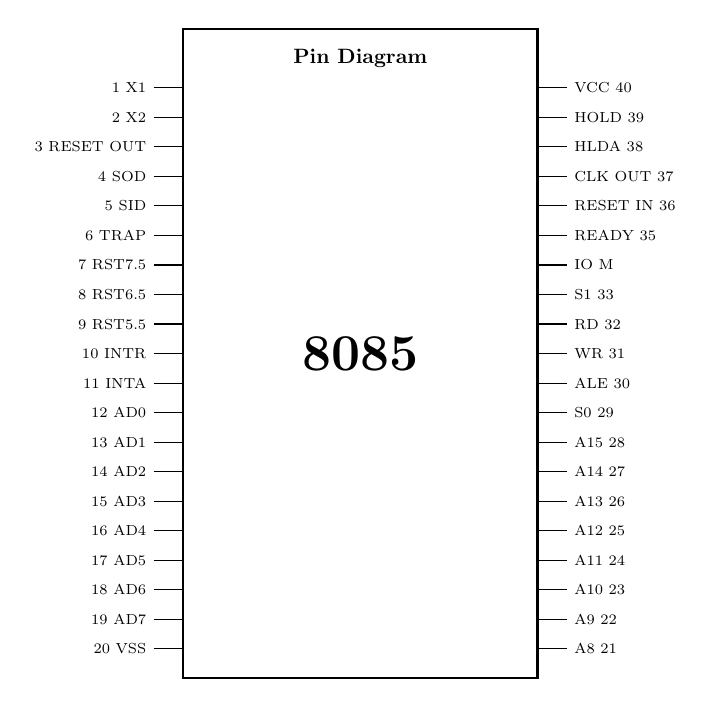
\begin{tikzpicture}[scale=0.75, transform shape]
    \draw [thick] (0,0) rectangle (6,11);
    \node at (3,5.5) {\Huge \textbf{8085}};
    \node at (3,10.5) {\textbf{Pin Diagram}};
    
    % Left Pins
    \foreach \y/\label/\pin in {10/X1/1, 9.5/X2/2, 9/RESET OUT/3, 8.5/SOD/4, 8/SID/5, 7.5/TRAP/6, 7/RST7.5/7, 6.5/RST6.5/8, 6/RST5.5/9, 5.5/INTR/10, 5/INTA/11, 4.5/AD0/12, 4/AD1/13, 3.5/AD2/14, 3/AD3/15, 2.5/AD4/16, 2/AD5/17, 1.5/AD6/18, 1/AD7/19, 0.5/VSS/20}
        \draw (-0.5, \y) node[left] {\scriptsize \pin\ \label} -- (0, \y);
        
    % Right Pins
    \foreach \y/\label/\pin in {10/VCC/40, 9.5/HOLD/39, 9/HLDA/38, 8.5/CLK OUT/37, 8/RESET IN/36, 7.5/READY/35, 7/IO/M/34, 6.5/S1/33, 6/RD/32, 5.5/WR/31, 5/ALE/30, 4.5/S0/29, 4/A15/28, 3.5/A14/27, 3/A13/26, 2.5/A12/25, 2/A11/24, 1.5/A10/23, 1/A9/22, 0.5/A8/21}
        \draw (6, \y) -- (6.5, \y) node[right] {\scriptsize \label\ \pin};
\end{tikzpicture}
\captionof{figure}{8085 Pin Diagram}
\end{center}
\end{solutionbox}

\begin{mnemonicbox}
\mnemonic{Address Data Control Power Interrupt (ADCPI)}
\end{mnemonicbox}

\questionmarks{2(a) OR}{3}{Explain Instruction Fetching Operation in 8085.}

\begin{solutionbox}
Instruction fetching is the first step in instruction cycle:

\begin{itemize}
    \item \textbf{PC contents} placed on address bus (A0-A15).
    \item \textbf{ALE signal} goes high to latch address.
    \item \textbf{RD signal} goes low to read memory.
    \item \textbf{Instruction} fetched from memory to data bus.
    \item \textbf{PC incremented} to point to next instruction.
\end{itemize}

This occurs during \textbf{T1 and T2} states and takes \textbf{4 clock cycles} for simple instructions.
\end{solutionbox}

\begin{mnemonicbox}
\mnemonic{PC ALE RD Fetch Increment (PARFI)}
\end{mnemonicbox}

\questionmarks{2(b) OR}{4}{Explain Flag Register of 8085.}

\begin{solutionbox}
The Flag Register stores status information after arithmetic/logical operations.

\begin{center}
\captionof{table}{8085 Flags}
\begin{tabulary}{\linewidth}{|L|L|L|}
\hline
\textbf{Bit} & \textbf{Flag} & \textbf{Function} \\ \hline
\textbf{D7} & \textbf{S (Sign)} & Set if result is negative \\ \hline
\textbf{D6} & \textbf{Z (Zero)} & Set if result is zero \\ \hline
\textbf{D4} & \textbf{AC (Aux Carry)} & Set if carry from bit 3 to 4 \\ \hline
\textbf{D2} & \textbf{P (Parity)} & Set if result has even parity \\ \hline
\textbf{D0} & \textbf{CY (Carry)} & Set if carry/borrow generated \\ \hline
\end{tabulary}
\end{center}

\begin{center}
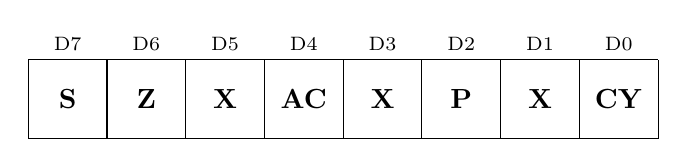
\begin{tikzpicture}
    \draw (0,0) grid (8,1);
    \foreach \x/\label in {0.5/S, 1.5/Z, 2.5/X, 3.5/AC, 4.5/X, 5.5/P, 6.5/X, 7.5/CY}
        \node at (\x, 0.5) {\textbf{\label}};
    \foreach \x/\bit in {0.5/D7, 1.5/D6, 2.5/D5, 3.5/D4, 4.5/D3, 5.5/D2, 6.5/D1, 7.5/D0}
        \node [above] at (\x, 1) {\scriptsize \bit};
\end{tikzpicture}
\captionof{figure}{Flag Register Format}
\end{center}
\end{solutionbox}

\begin{mnemonicbox}
\mnemonic{S-Z-X-AC-X-P-X-CY}
\end{mnemonicbox}

\questionmarks{2(c) OR}{7}{Explain Architecture of 8085 with neat sketch.}

\begin{solutionbox}
The 8085 architecture consists of ALU, Registers, Control Unit, and Buses.

\begin{center}
\begin{tikzpicture}[scale=0.85, transform shape]
    % Main Blocks
    \node [gtu block] (alu) {ALU};
    \node [gtu block, below=1cm of alu] (acc) {Accumulator};
    \node [gtu block, right=1cm of acc] (flags) {Flags};
    \node [gtu block, right=2.5cm of alu, minimum width=2.5cm] (regs) {Registers\\B,C, D,E, H,L\\SP, PC};
    \node [gtu block, below=1cm of acc] (control) {Timing \&\\Control Unit};
    
    % Buses
    \draw [->, thick] (regs.east) -- ++(1,0) node[right] {Address/Data Bus};
    \draw [->, thick] (control.south) -- ++(0,-1) node[below] {Control Signals};
    
    % Connections
    \draw [gtu arrow, <->] (alu) -- (acc);
    \draw [gtu arrow] (alu) -- (flags);
    \draw [gtu arrow, <->] (alu) -- (regs);
    \draw [gtu arrow] (control) -| (regs);
    \draw [gtu arrow] (control) -- (acc);
    \draw [gtu arrow] (control) -- (alu);
\end{tikzpicture}
\captionof{figure}{8085 Architecture}
\end{center}

\begin{itemize}
    \item \textbf{ALU}: Performs arithmetic and logical operations.
    \item \textbf{Registers}: Store data (A, B, C...) and addresses (PC, SP) temporarily.
    \item \textbf{Control Unit}: Generates signals (RD, WR, ALE) for operation.
    \item \textbf{Buses}: Address (16-bit) and Data (8-bit) buses for communication.
\end{itemize}
\end{solutionbox}

\begin{mnemonicbox}
\mnemonic{ALU Registers Control Address Data (ARCAD)}
\end{mnemonicbox}

\questionmarks{3(a)}{3}{Explain Internal RAM Organization of 8051 Microcontroller.}

\begin{solutionbox}
The 8051 has 128 bytes of internal RAM organized as:

\begin{center}
\captionof{table}{RAM Organization}
\begin{tabulary}{\linewidth}{|L|L|}
\hline
\textbf{Address} & \textbf{Purpose} \\ \hline
\textbf{00H-1FH} & Register Banks (4 banks of 8 registers each) \\ \hline
\textbf{20H-2FH} & Bit Addressable Area (16 bytes) \\ \hline
\textbf{30H-7FH} & General Purpose RAM (80 bytes) \\ \hline
\end{tabulary}
\end{center}

\begin{center}
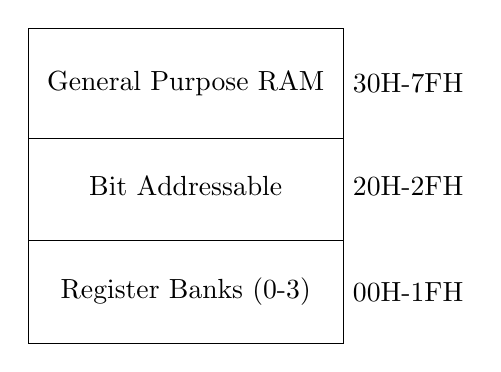
\begin{tikzpicture}
    \draw (0,0) rectangle (4,4);
    \draw (0,1.3) -- (4,1.3);
    \draw (0,2.6) -- (4,2.6);
    
    \node at (2, 3.3) {General Purpose RAM};
    \node [right] at (4,3.3) {30H-7FH};
    
    \node at (2, 2) {Bit Addressable};
    \node [right] at (4,2) {20H-2FH};
    
    \node at (2, 0.65) {Register Banks (0-3)};
    \node [right] at (4,0.65) {00H-1FH};
\end{tikzpicture}
\captionof{figure}{Internal RAM Map}
\end{center}
\end{solutionbox}

\begin{mnemonicbox}
\mnemonic{Register Bit General (RBG)}
\end{mnemonicbox}

\questionmarks{3(b)}{4}{Explain Function of Each bit of TMOD SFR of 8051 Microcontroller.}

\begin{solutionbox}
TMOD (Timer Mode) register controls Timer 0 and Timer 1.

\begin{center}
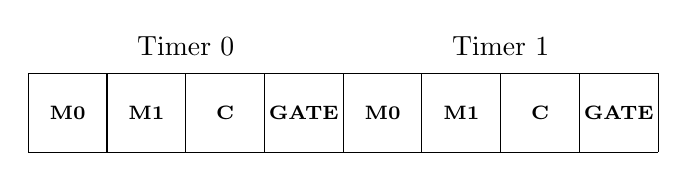
\begin{tikzpicture}
    \draw (0,0) grid (8,1);
    \foreach \x/\label in {0.5/M0, 1.5/M1, 2.5/C/T, 3.5/GATE, 4.5/M0, 5.5/M1, 6.5/C/T, 7.5/GATE}
        \node at (\x, 0.5) {\scriptsize \textbf{\label}};
    \node [above] at (2,1.1) {Timer 0};
    \node [above] at (6,1.1) {Timer 1};
\end{tikzpicture}
\captionof{figure}{TMOD Register}
\end{center}

\begin{itemize}
    \item \textbf{GATE}: 1 = External gate control (INTx pin), 0 = Internal control.
    \item \textbf{C/T}: 1 = Counter mode, 0 = Timer mode.
    \item \textbf{M1, M0}: Mode selection (00: 13-bit, 01: 16-bit, 10: 8-bit auto-reload, 11: Split).
\end{itemize}
\end{solutionbox}

\begin{mnemonicbox}
\mnemonic{GATE C/T Mode1 Mode0}
\end{mnemonicbox}

\questionmarks{3(c)}{7}{Explain Architecture of 8051 with neat sketch.}

\begin{solutionbox}
The 8051 has Harvard architecture with separate program and data memory.

\begin{center}
\begin{tikzpicture}[scale=0.9, transform shape]
    \node [gtu block, minimum height=3cm, minimum width=2cm] (cpu) {CPU};
    \node [gtu block, right=2cm of cpu] (rom) {4KB ROM};
    \node [gtu block, below=0.5cm of rom] (ram) {128B RAM};
    \node [gtu block, left=2cm of cpu] (timers) {Timer 0/1};
    \node [gtu block, below=0.5cm of timers] (serial) {Serial Port};
    \node [gtu block, above=1cm of cpu] (int) {Interrupts};
    \node [gtu block, below=2cm of cpu, minimum width=6cm] (ports) {I/O Ports P0, P1, P2, P3};
    
    \draw [thick, <->] (cpu) -- (rom);
    \draw [thick, <->] (cpu) -- (ram);
    \draw [thick, <->] (cpu) -- (timers);
    \draw [thick, <->] (cpu) -- (serial);
    \draw [thick, <->] (cpu) -- (int);
    \draw [thick, <->] (cpu) -- (ports);
\end{tikzpicture}
\captionof{figure}{8051 Architecture}
\end{center}

\begin{itemize}
    \item \textbf{Memory}: 4KB ROM (Program), 128B RAM (Data).
    \item \textbf{Peripherals}: 4 I/O Ports, 2 Timers, 1 Serial Port.
    \item \textbf{Interrupts}: 5 Sources (External, Timer, Serial).
\end{itemize}
\end{solutionbox}

\begin{mnemonicbox}
\mnemonic{CPU ROM RAM Ports Timers Serial Interrupts (CRRRPTI)}
\end{mnemonicbox}

\questionmarks{3(a) OR}{3}{Explain PSW SFR of 8051 Microcontroller.}

\begin{solutionbox}
PSW (Program Status Word) contains status flags.

\begin{center}
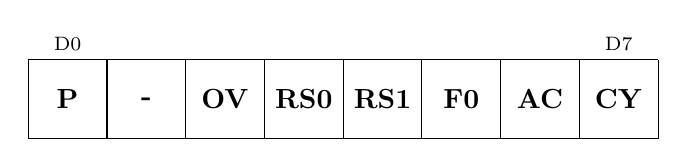
\begin{tikzpicture}
    \draw (0,0) grid (8,1);
    \foreach \x/\label in {0.5/P, 1.5/-, 2.5/OV, 3.5/RS0, 4.5/RS1, 5.5/F0, 6.5/AC, 7.5/CY}
        \node at (\x, 0.5) {\textbf{\label}};
    \node [above] at (7.5, 1) {\scriptsize D7}; \node [above] at (0.5, 1) {\scriptsize D0};
\end{tikzpicture}
\captionof{figure}{PSW Register}
\end{center}

\begin{itemize}
    \item \textbf{CY}: Carry Flag. \textbf{AC}: Aux Carry.
    \item \textbf{RS1, RS0}: Register Bank Select (00-Bank0, 01-Bank1, 10-Bank2, 11-Bank3).
    \item \textbf{OV}: Overflow Flag. \textbf{P}: Parity Flag.
\end{itemize}
\end{solutionbox}

\begin{mnemonicbox}
\mnemonic{CY AC F0 RS1 RS0 OV - P}
\end{mnemonicbox}

\questionmarks{3(b) OR}{4}{Explain Function of Each bit of SCON SFR of 8051 Microcontroller.}

\begin{solutionbox}
SCON controls serial communication.

\begin{center}
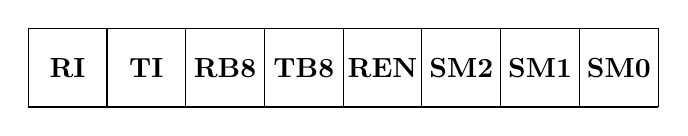
\begin{tikzpicture}
    \draw (0,0) grid (8,1);
    \foreach \x/\label in {0.5/RI, 1.5/TI, 2.5/RB8, 3.5/TB8, 4.5/REN, 5.5/SM2, 6.5/SM1, 7.5/SM0}
        \node at (\x, 0.5) {\textbf{\label}};
\end{tikzpicture}
\captionof{figure}{SCON Register}
\end{center}

\begin{itemize}
    \item \textbf{SM0, SM1}: Mode selection (0-Shi.Reg, 1-8bit UART, 2-9bit Fixed, 3-9bit Var).
    \item \textbf{REN}: Receive Enable.
    \item \textbf{TB8/RB8}: 9th bit for transmit/receive.
    \item \textbf{TI/RI}: Transmit/Receive Interrupt flags.
\end{itemize}
\end{solutionbox}

\begin{mnemonicbox}
\mnemonic{SM0 SM1 SM2 REN TB8 RB8 TI RI}
\end{mnemonicbox}

\questionmarks{3(c) OR}{7}{Explain Pin Diagram of 8051 with neat sketch.}

\begin{solutionbox}
The 8051 is a 40-pin DIP package.

\begin{center}
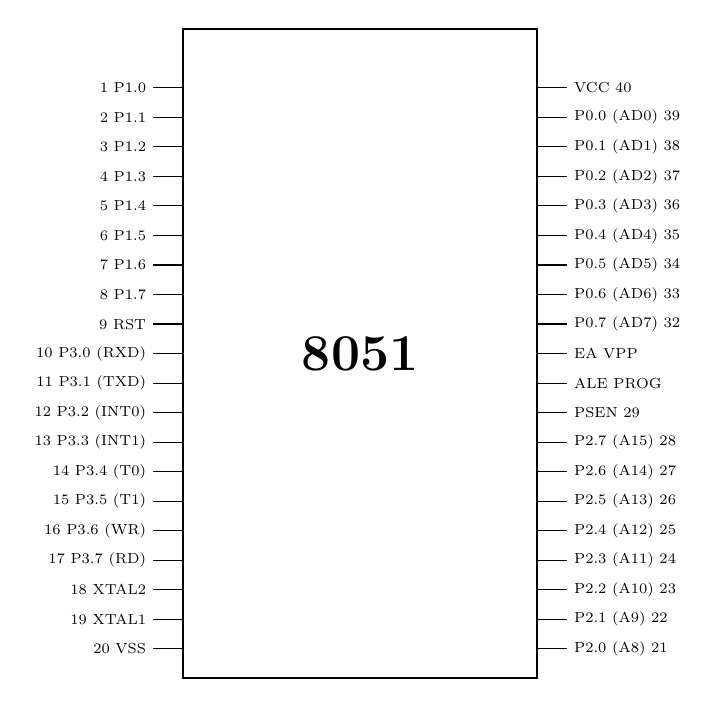
\begin{tikzpicture}[scale=0.75, transform shape]
    \draw [thick] (0,0) rectangle (6,11);
    \node at (3,5.5) {\Huge \textbf{8051}};
    
    % Left Pins (1-20)
    \foreach \y/\label/\pin in {10/P1.0/1, 9.5/P1.1/2, 9/P1.2/3, 8.5/P1.3/4, 8/P1.4/5, 7.5/P1.5/6, 7/P1.6/7, 6.5/P1.7/8, 6/RST/9, 5.5/P3.0 (RXD)/10, 5/P3.1 (TXD)/11, 4.5/P3.2 (INT0)/12, 4/P3.3 (INT1)/13, 3.5/P3.4 (T0)/14, 3/P3.5 (T1)/15, 2.5/P3.6 (WR)/16, 2/P3.7 (RD)/17, 1.5/XTAL2/18, 1/XTAL1/19, 0.5/VSS/20}
        \draw (-0.5, \y) node[left] {\scriptsize \pin\ \label} -- (0, \y);
        
    % Right Pins (40-21)
    \foreach \y/\label/\pin in {10/VCC/40, 9.5/P0.0 (AD0)/39, 9/P0.1 (AD1)/38, 8.5/P0.2 (AD2)/37, 8/P0.3 (AD3)/36, 7.5/P0.4 (AD4)/35, 7/P0.5 (AD5)/34, 6.5/P0.6 (AD6)/33, 6/P0.7 (AD7)/32, 5.5/EA/VPP/31, 5/ALE/PROG/30, 4.5/PSEN/29, 4/P2.7 (A15)/28, 3.5/P2.6 (A14)/27, 3/P2.5 (A13)/26, 2.5/P2.4 (A12)/25, 2/P2.3 (A11)/24, 1.5/P2.2 (A10)/23, 1/P2.1 (A9)/22, 0.5/P2.0 (A8)/21}
        \draw (6, \y) -- (6.5, \y) node[right] {\scriptsize \label\ \pin};
\end{tikzpicture}
\captionof{figure}{8051 Pin Diagram}
\end{center}

\begin{itemize}
    \item \textbf{Port 0}: Multiplexed AD0-AD7. \textbf{Port 2}: High Address A8-A15.
    \item \textbf{Port 1}: I/O only. \textbf{Port 3}: Special functions (RX, TX, INT, T0, T1, WR, RD).
    \item \textbf{Control}: RST, ALE, PSEN, EA.
\end{itemize}
\end{solutionbox}

\begin{mnemonicbox}
\mnemonic{Port Power Crystal Control (PPCC)}
\end{mnemonicbox}

\questionmarks{4(a)}{3}{Write and Explain any Three Data Transfer Instructions of 8051 Microcontroller.}

\begin{solutionbox}
\begin{center}
\captionof{table}{Data Transfer Instructions}
\begin{tabulary}{\linewidth}{|L|L|}
\hline
\textbf{Instruction} & \textbf{Function} \\ \hline
\code{MOV A, R0} & Move contents of R0 to Accumulator. \\ \hline
\code{MOV R1, \#50H} & Move immediate data 50H to R1. \\ \hline
\code{MOV 30H, A} & Move Accumulator contents to direct address 30H. \\ \hline
\end{tabulary}
\end{center}

\begin{lstlisting}[language={[x86masm]Assembler}, caption={Data Transfer Examples}]
MOV A, R0       ; A = R0
MOV R1, #50H    ; R1 = 50H
MOV 30H, A      ; [30H] = A
\end{lstlisting}
\end{solutionbox}

\begin{mnemonicbox}
\mnemonic{MOV Between Register Immediate Direct}
\end{mnemonicbox}

\questionmarks{4(b)}{4}{Write 8051 Assembly Language Program to Multiply Content of R0 and R1 and Store Result in R5 (Lower Byte) and R6 (Higher Byte).}

\begin{solutionbox}
\begin{lstlisting}[language={[x86masm]Assembler}, caption={Multiplication Program}]
    ORG 0000H
    
    MOV A, R0       ; Load Multiplicand
    MOV B, R1       ; Load Multiplier
    MUL AB          ; Multiply A * B
                    ; Result: B(High) A(Low)
    
    MOV R5, A       ; Store Lower Byte
    MOV R6, B       ; Store Higher Byte
    
    SJMP $          ; Stop
    END
\end{lstlisting}
\end{solutionbox}

\questionmarks{4(c)}{7}{List Addressing Modes of 8051 Microcontroller and Explain each with Example.}

\begin{solutionbox}
\begin{center}
\captionof{table}{Addressing Modes}
\begin{tabulary}{\linewidth}{|L|L|L|}
\hline
\textbf{Mode} & \textbf{Description} & \textbf{Example} \\ \hline
\textbf{Immediate} & Data directly in instruction (\#). & \code{MOV A, \#50H} \\ \hline
\textbf{Register} & Data in register (Rn). & \code{MOV A, R0} \\ \hline
\textbf{Direct} & Data at direct memory address. & \code{MOV A, 30H} \\ \hline
\textbf{Indirect} & Address in register (@Ri). & \code{MOV A, @R0} \\ \hline
\textbf{Indexed} & Base + Offset (usually for ROM). & \code{MOVC A, @A+DPTR} \\ \hline
\textbf{Relative} & Offset added to PC (Jumps). & \code{SJMP LABEL} \\ \hline
\textbf{Bit} & Direct bit address. & \code{SETB P1.0} \\ \hline
\end{tabulary}
\end{center}
\end{solutionbox}

\begin{mnemonicbox}
\mnemonic{Immediate Register Direct Indirect Indexed Relative Bit (I-R-D-I-I-R-B)}
\end{mnemonicbox}

\questionmarks{4(a) OR}{3}{Write and Explain any Three Logical Instructions 8051 Microcontroller.}

\begin{solutionbox}
\begin{center}
\captionof{table}{Logical Instructions}
\begin{tabulary}{\linewidth}{|L|L|}
\hline
\textbf{Instruction} & \textbf{Function} \\ \hline
\code{ANL A, R0} & AND Accumulator with R0. Masking bits. \\ \hline
\code{ORL A, \#0FH} & OR Accumulator with immediate 0FH. Setting bits. \\ \hline
\code{XRL A, 30H} & XOR Accumulator with memory. Toggling bits. \\ \hline
\end{tabulary}
\end{center}

\begin{lstlisting}[language={[x86masm]Assembler}, caption={Logical Examples}]
ANL A, R0       ; A = A AND R0
ORL A, #0FH     ; A = A OR 0FH
XRL A, 30H      ; A = A XOR [30H]
\end{lstlisting}
\end{solutionbox}

\questionmarks{4(b) OR}{4}{Write 8051 Assembly Language Program to Subtract Number Stored in 2000h from 2001h and Store result in 2002h. (External Memory).}

\begin{solutionbox}
\begin{lstlisting}[language={[x86masm]Assembler}, caption={Subtraction Program}]
    ORG 0000H
    
    MOV DPTR, #2001H    ; Point to Minuend
    MOVX A, @DPTR       ; Load Minuend
    MOV R0, A           ; Save in R0
    
    MOV DPTR, #2000H    ; Point to Subtrahend
    MOVX A, @DPTR       ; Load Subtrahend
    MOV R1, A           ; Save in R1
    
    MOV A, R0           ; Restore Minuend
    CLR C               ; Clear Carry for SUBB
    SUBB A, R1          ; A = Minuend - Subtrahend
    
    MOV DPTR, #2002H    ; Point to Result
    MOVX @DPTR, A       ; Store Result
    
    SJMP $
    END
\end{lstlisting}
\end{solutionbox}

\questionmarks{4(c) OR}{7}{Explain Instructions: RET, PUSH, CLR PSW.0, RLC A, CJNE, NOP, ANL.}

\begin{solutionbox}
\begin{center}
\captionof{table}{Instruction Explanation}
\begin{tabulary}{\linewidth}{|L|L|}
\hline
\textbf{Instruction} & \textbf{Function} \\ \hline
\code{RET} & Return from subroutine. Pops PC from stack. \\ \hline
\code{PUSH 30H} & Pushes contents of address 30H onto Stack. \\ \hline
\code{CLR PSW.0} & Clears Carry Flag (Bit 0 of PSW). \\ \hline
\code{RLC A} & Rotate A Left through Carry Flag. \\ \hline
\code{CJNE A, \#dat, L} & Compare A with data, Jump to Label if Not Equal. \\ \hline
\code{NOP} & No Operation. Consumes time/space only. \\ \hline
\code{ANL A, \#data} & Logical AND Accumulator with immediate data. \\ \hline
\end{tabulary}
\end{center}
\end{solutionbox}

\begin{mnemonicbox}
\mnemonic{Return Push Clear Rotate Compare No-op AND}
\end{mnemonicbox}

\questionmarks{5(a)}{3}{List the application of Microcontroller in various fields.}

\begin{solutionbox}
\begin{center}
\captionof{table}{Applications}
\begin{tabulary}{\linewidth}{|L|L|}
\hline
\textbf{Field} & \textbf{Applications} \\ \hline
\textbf{Consumer} & TV Remotes, Washing Machines, Microwaves \\ \hline
\textbf{Automotive} & ABS, Engine Control, Airbags \\ \hline
\textbf{Industrial} & Robotics, Process Control, Automation \\ \hline
\textbf{Medical} & Pacemakers, Glucose Meters \\ \hline
\textbf{Communication} & Mobile Phones, Modems \\ \hline
\textbf{Home} & Smart Thermostats, Security Systems \\ \hline
\end{tabulary}
\end{center}
\end{solutionbox}


\questionmarks{5(b)}{4}{Interface Stepper Motor with 8051 Microcontroller and Explain in brief.}

\begin{solutionbox}
Stepper motor requires a driver like ULN2003 for current amplification.

\begin{center}
\begin{circuitikz}[scale=0.9, transform shape]
    \node [gtu block, minimum height=3cm] (cpu) {8051\\(P1)};
    \node [gtu block, right=2cm of cpu] (uln) {ULN2003\\Driver};
    \node [gtu block, right=2cm of uln] (motor) {Stepper\\Motor};
    
    \draw [->, thick] ($(cpu.east)+(0,0.5)$) -- node[above] {P1.0-P1.3} ($(uln.west)+(0,0.5)$);
    \draw [->, thick] ($(uln.east)+(0,0.5)$) -- node[above] {Coils A-D} ($(motor.west)+(0,0.5)$);
    
    \node [below=0.5cm of uln] {12V Supply};
    \draw [->] (4, -2) -- (uln.south);
\end{circuitikz}
\captionof{figure}{Stepper Motor Interface}
\end{center}

\begin{center}
\captionof{table}{Half-Step Sequence}
\begin{tabulary}{\linewidth}{|C|C|C|C|C|C|}
\hline
\textbf{Step} & \textbf{P1.3} & \textbf{P1.2} & \textbf{P1.1} & \textbf{P1.0} & \textbf{Hex} \\ \hline
1 & 0 & 0 & 0 & 1 & 01H \\ \hline
2 & 0 & 0 & 1 & 1 & 03H \\ \hline
3 & 0 & 0 & 1 & 0 & 02H \\ \hline
4 & 0 & 1 & 1 & 0 & 06H \\ \hline
\end{tabulary}
\end{center}
\end{solutionbox}

\begin{mnemonicbox}
\mnemonic{Step Sequence Driver Protection (SSDP)}
\end{mnemonicbox}

\questionmarks{5(c)}{7}{Draw interfacing circuit to interface 4 LED at port 2.0 to 2.3 of microcontroller 8051 and write assembly language program to flash it.}

\begin{solutionbox}
\begin{center}
\begin{circuitikz}
    \node [draw, minimum height=2.5cm] (p2) {8051 P2};
    \foreach \y/\p in {1/P2.0, 0.5/P2.1, 0/P2.2, -0.5/P2.3} {
        \draw (p2.east) ++(0,\y) -- ++(1,0) to[R, l=330$\Omega$] ++(1.5,0) to[leDo] ++(1,0) node[ground]{};
        \node at ($(p2.east)+(-0.8,\y)$) {\scriptsize \p};
    }
\end{circuitikz}
\captionof{figure}{4 LED Interface}
\end{center}

\begin{lstlisting}[language={[x86masm]Assembler}, caption={LED Flashing Program}]
    ORG 0000H
MAIN:
    MOV P2, #0FH        ; Turn ON LEDs (P2.0-P2.3 = 1)
    ACALL DELAY
    MOV P2, #00H        ; Turn OFF LEDs
    ACALL DELAY
    SJMP MAIN
    
DELAY:
    MOV R0, #255
L1: MOV R1, #255
L2: DJNZ R1, L2
    DJNZ R0, L1
    RET
    END
\end{lstlisting}
\end{solutionbox}

\begin{mnemonicbox}
\mnemonic{Resistor LED Ground Program (RLGP)}
\end{mnemonicbox}

\questionmarks{5(a) OR}{3}{Draw Interfacing of Push button switch and LED with 8051 Microcontroller.}

\begin{solutionbox}
Switch at P1.0 (Input), LED at P1.1 (Output).

\begin{center}
\begin{circuitikz}
    % Switch
    \draw (0,2) node[vcc] {+5V} to[R, l=10k$\Omega$] (0,1) -- (0,-0.5) to[push button, l=Sw] (0,-1.5) node[ground]{};
    \draw (0,1) -- (1.5,1) node[right] {P1.0 (Input)};
    
    % LED
    \draw (4,1) node[left] {P1.1 (Output)} to[R, l=330$\Omega$] (5.5,1) to[leDo] (7,1) node[ground]{};
\end{circuitikz}
\captionof{figure}{Switch and LED Interface}
\end{center}
\end{solutionbox}

\begin{mnemonicbox}
\mnemonic{Pull-up Switch LED Current-limit (PSLC)}
\end{mnemonicbox}

\questionmarks{5(b) OR}{4}{Interface Relay with 8051 Microcontroller and Explain in brief.}

\begin{solutionbox}
Relay is an electromechanical switch. It isolates high voltage load from microcontroller.

\begin{center}
\begin{circuitikz}
    \draw (0,0) node[left] {P1.0} to[R, l=1k$\Omega$] (2,0) node[npn, anchor=B] (Q) {BC547};
    \draw (Q.E) node[ground]{} -- (2,0); % Emitter to GND
    
    % Relay Coil
    \draw (Q.C) -- (2,2) to[L, l=Relay] (2,3.5) node[vcc] {+12V};
    
    % Flyback Diode
    \draw (3,2) to[D*, l=1N4007] (3,3.5);
    \draw (2,2) -- (3,2);
    \draw (2,3.5) -- (3,3.5);
    
    % Contacts
    \draw (2.5, 2.8) -- (4, 2.8) node[right] {NO};
    \draw (4, 2.6) node[right] {COM};
\end{circuitikz}
\captionof{figure}{Relay Driver Circuit}
\end{center}

\begin{itemize}
    \item \textbf{Transistor}: Acts as switch. P1.0=1 $\rightarrow$ Transistor ON $\rightarrow$ Relay ON.
    \item \textbf{Flyback Diode}: Protects transistor from back EMF.
    \item \textbf{Isolation}: High voltage AC load is isolated from 5V logic.
\end{itemize}
\end{solutionbox}

\begin{mnemonicbox}
\mnemonic{Transistor Resistor Diode Relay (TRDR)}
\end{mnemonicbox}

\questionmarks{5(c) OR}{7}{Interface 7 segment LED with 8051 Microcontroller and write assembly language program to print 0 on it.}

\begin{solutionbox}
Common Cathode display connected to Port 1.

\begin{center}
\begin{circuitikz}
    \node [draw, minimum size=2cm] (disp) {7-Seg};
    \node [left=2cm of disp] (p1) {Port 1};
    
    \draw [->] (p1) -- node[above] {a-g, dp} (disp);
    \draw (disp.south) -- ++(0,-0.5) node[ground] {};
    
    \node [right=0.2cm of disp] {\scriptsize a=P1.0 ... dp=P1.7};
\end{circuitikz}
\captionof{figure}{7-Segment Connection}
\end{center}

\begin{center}
\captionof{table}{Digit 0 Code}
\begin{tabulary}{\linewidth}{|C|C|C|}
\hline
\textbf{Digit} & \textbf{Segments (gfedcba)} & \textbf{Hex} \\ \hline
0 & 0 1 1 1 1 1 1 & 3FH \\ \hline
\end{tabulary}
\end{center}

\begin{lstlisting}[language={[x86masm]Assembler}, caption={Display 0}]
    ORG 0000H
MAIN:
    MOV P1, #3FH        ; Pattern for '0'
    SJMP MAIN           ; Loop
    END
\end{lstlisting}
\end{solutionbox}

\begin{mnemonicbox}
\mnemonic{Seven Segments Common Cathode Current-limit (SSCCC)}
\end{mnemonicbox}

\end{document}
